\subsection{Dilations and Reflections}

\begin{tcolorbox}[title=Problem 2, breakable]
    Let $A$ be a point, $A \ne 0$. If $b, c$ are numbers 
    such that $b A = c A$, prove that $b = c$.
\end{tcolorbox}

\begin{proof}
    Let $A = (a_1, a_2)$. Then $b A = (b a_1, b a_2)$
        and $c A = (c a_1, c a_2)$.
    Suppose $b A = c A$.
    Then $b a_1 = c a_1$ and $b a_2 = c a_2$.
    Since $A \ne 0$ either $a_1 \ne 0$ or $a_2 \ne 0$.
    Suppose $a_1 \ne 0$ then since $b a_1 = c a_1$
        dividing by $a_1$ shows $b = c$.
    Suppose $a_2 \ne 0$ then since $b a_2 = c a_2$
        dividing by $a_2$ shows $b = c$.

    Therefore $b = c$.
\end{proof}

\begin{tcolorbox}[title=Problem 3, breakable]
    Prove that reflection through $O$ preserves distances.
    In other words, prove that 
    \[d(A, B) = d(-A, -B)\]
\end{tcolorbox}

\begin{proof}
    Let $A = (a_1, a_2)$ and $B = (b_1, b_2)$. Then
    \[
    d(-A, -B) = \sqrt{((-a_1)-(-b_1))^2 + ((-a_2)-(-b_2))^2}
    = \sqrt{(a_1 - b_1)^2 + (a_2 - b_2)^2} = d(A, B).
    \]
\end{proof}

\begin{tcolorbox}[title=Problem 4, breakable]
    \textbf{The $3-$ dimensional case}

    (a) Define the multiplication (dilation) of a point $A = (a_1, a_2, a_3)$
        by a number $c$. Write out interpretations for this similar to those 
        we did in the plane. Draw pictures.

    (b) Define reflection $A$ through $O = (0, 0, 0)$.

    (c) State and prove the analogs of Theorems $1$ and $2$.
\end{tcolorbox}
\begin{figure}[h]
    \centering
    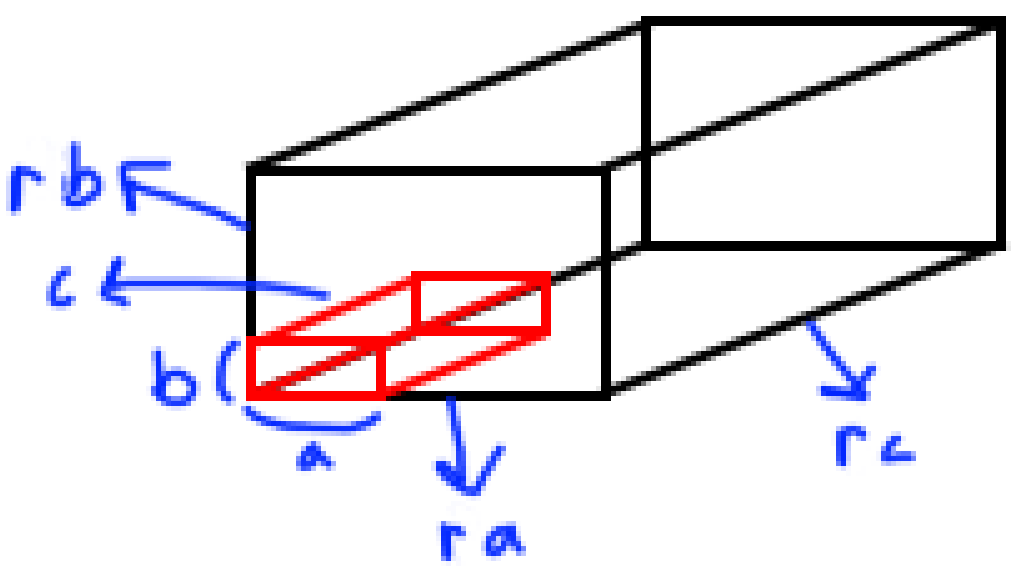
\includegraphics[width=0.6\textwidth]{images/arb2_rect.png}
\end{figure}
\begin{definition}
    Let $r$ be a real number.
    Let the dilation of a point $A = (a_1, a_2, a_3)$ by $r$ be defined as follows
    \[r A = (r a_1, r a_2, r a_3)\]
\end{definition}
\begin{definition}
    Let the reflection $R$ of $A$ through $O = (0, 0, 0)$
    dilation with $r = -1$.
\end{definition}
\begin{theorem}
    Let $r$ be a postiive number. If $A, B$ are points, then 
    \[d(A, B) = r \cdot d(A, B)\]
\end{theorem}
\begin{proof}
    Let $A = (a_1, a_2, a_3)$ and $B = (b_1, b_2, b_3)$.
    Then $r A = (r a_1, r a_2, r a_3)$ and $r B = (r b_1, r b_2, r b_3)$.
    Hence 
    \begin{align*}
        d(r A, r B)^2 
            &= (r b_1 - r a_1)^2 + (r b_2 - r a_2)^2 + (r b_3 - r a_3)^2 \\
            &= (r (b_1 - a_1))^2 + (r (b_2 - a_2))^2 + (r (b_3 - a_3))^2 \\
            &= r^2(b_1 - a_1)^2 + r^2(b_2 - a_2)^2 + r^2(b_3 - a_3)^2 \\
            &= r^2 \cdot d(A, B)^2
    \end{align*}
    Taking the square root proves our theorem.
\end{proof}
\begin{theorem}
    Let $c$ be a number. Then 
    \[d(c A, c B) = |c| \cdot d(A, B)\]
\end{theorem}
\begin{proof}
    Let $A = (a_1, a_2, a_3)$ and $B = (b_1, b_2, b_3)$.
    Then $c A = (c a_1, c a_2, c a_3)$ and $c B = (c b_1, c b_2, c b_3)$.
    Hence 
    \begin{align*}
        d(c A, c B)^2 
            &= (c b_1 - c a_1)^2 + (c b_2 - c a_2)^2 + (c b_3 - c a_3)^2 \\
            &= (c (b_1 - a_1))^2 + (c (b_2 - a_2))^2 + (c (b_3 - a_3))^2 \\
            &= c^2(b_1 - a_1)^2 + c^2(b_2 - a_2)^2 + c^2(b_3 - a_3)^2 \\
            &= c^2 \cdot d(A, B)^2
    \end{align*}
    Taking the square root proves our theorem since $\sqrt{c^2} = |c|$.
\end{proof}

\subsection{Addition, Subtraction, and Parallelogram Law}

\begin{tcolorbox}[title=Problem 11, breakable]
    Let $T_A$ be a translation by $A$. Prove that it is an isometry,
    in other words, that for any pair of points $P, Q$ we have 
    \[d(P, Q) = d(T_A(P), T_A(Q))\]
\end{tcolorbox}

\begin{proof}
    Let $P = (p_1, p_2), Q = (q_1, q_2), A = (a_1, a_2)$.
    Now $d(P, Q) = \sqrt{(p_1 - q_1)^2 + (p_2 - q_2)^2}$.
    Then $d(T_A(P), T_A(Q)) 
        = \sqrt{((p_1 + a_1)^2 - (q_1 + a_1)^2) + ((p_2 + a_2) - (q_2 + a_2))^2}
        = \sqrt{(p_1^2 + 2 p_1 a_1 + a_1^2 - q_1^2 - 2 q_1 a_1 - a_1^2) + ()} $.
\end{proof}

\begin{tcolorbox}[title=Problem 12, breakable]
    Let $D(r, A)$ denote the disc of radius $r$ centered at $A$.
    Show that $D(r, A)$ is the translation of $A$ of the disc $D(r, O)$
    of radius $r$ centered at $O$.
\end{tcolorbox}

\begin{tcolorbox}[title=Problem 13, breakable]
    Let $S(r, P)$ denote the circle of radius $r$ centered at $P$.

    (a) Show that the reflection of this circle through $O$ is a again a circle.
        What is the center of the reflected circle.

    (b) Show that the reflection of the disc $D(r, P)$ through $O$ is a disc.
        What is the center of this reflected disc?
\end{tcolorbox}

\begin{tcolorbox}[title=Problem 14, breakable]
    Let $P, Q$ be points. Write $P = Q + A$, where $A = P - Q$. Define 
    the \textbf{reflection of $P$ through $Q$} to be the point $Q - A$.
    If $R_Q$ denotes reflection through $Q$, tehn we have $R_Q(P) = 2 Q - P$.
    (Why?) Draw the picture, showing $P, Q, A$ and $Q - A$ to convince yourself
    that this definition corresponds to our geometric intuition.
\end{tcolorbox}

\begin{tcolorbox}[title=Problem 15, breakable]
    (a) Prove that reflection through a point $Q$ can be expressed in terms 
        of reflection through $O$, followed by a translation.

    (b) Let $T_A$ be translation by $A$, and $R_0$ reflection with respect 
        to teh origin. PRove that the composite $T_A \circ R_0$ is equal 
        to $R_Q$ for some point $Q$. Which one?
\end{tcolorbox}

\begin{tcolorbox}[title=Problem 16, breakable]
    (a) Let $r$ be a positive number.
        Give an analytic definition of \textbf{dilation by $r$ with respect to a point $Q$},
        and denote this dilation by $F_{r, Q}$. To give this definition, look at 
        Excersize $14$. You may also want to look at the discussion about line segments
        in $4$. If $P$ is a point, draw the picture with $O, P, Q, P - Q$, and $F_{r, Q}(P)$.

    (b) From your definition, it should be clear that $F_{r, Q}$ can be obtained as a composite 
        of dilation with respect to $O$, and a translation. Translation by what point?
\end{tcolorbox}

\begin{tcolorbox}[title=Problem 17, breakable]
    Let $S(r, A)$ be the circle of radius $r$ and center $A$.
    Show that the reflection of this circle through a point $Q$ is a circle.
    What is the center of this reflected circle?
    What is its radius?
    Draw a picture.
\end{tcolorbox}

\begin{tcolorbox}[title=Problem 18, breakable]
    The inverse of the translation $T_A$ is also a translation.
    By what? Prove your assertion.
\end{tcolorbox}

\begin{tcolorbox}[title=Problem 19, breakable]
    Let $F_r$ be dilation by a postive number $r$,
    with respect to $O$, and let $T_A$ be a translation by $A$.

    (a) Show that $F_r^{-1}$ is also a dilation. By what number?

    (c) Show that $F_R \circ T_A \circ F_r^{-1}$ is a translation.
\end{tcolorbox}

\begin{tcolorbox}[title=Problem 20, breakable]
    Show that the composite of two translations is a translation.
    $T_A \circ T_B = T_C$, how would you express $C$ in terms 
    of $A$ and $B$?
\end{tcolorbox}

\begin{tcolorbox}[title=Problem 21, breakable]
    Let $R$ be a reflection through the origin.

    (a) Show that $R^{-1}$ exists.

    (b) Show that $R \circ T_A \circ R^{-1}$ is a translation. By what?
\end{tcolorbox}

\begin{tcolorbox}[title=Problem 22, breakable]
\end{tcolorbox}

\begin{tcolorbox}[title=Problem 23, breakable]
\end{tcolorbox}

\begin{tcolorbox}[title=Problem 24, breakable]
\end{tcolorbox}

\begin{tcolorbox}[title=Problem 25, breakable]
\end{tcolorbox}

\begin{tcolorbox}[title=Problem 26, breakable]
\end{tcolorbox}

\begin{tcolorbox}[title=Problem 29, breakable]
\end{tcolorbox}

\begin{tcolorbox}[title=Problem 30, breakable]
\end{tcolorbox}

\begin{tcolorbox}[title=Problem 31, breakable]
\end{tcolorbox}

\begin{tcolorbox}[title=Problem 32, breakable]
\end{tcolorbox}